\documentclass{article}

\usepackage[T1]{fontenc}
\usepackage[utf8]{inputenc}
\usepackage[swedish]{babel}
\usepackage{fullpage}
\usepackage{amssymb}
\usepackage{bussproofs}
\usepackage{amsmath}
\usepackage{graphicx}
\usepackage{verbatim}
\usepackage{tikz}
\let\emptyset\varnothing


\title{Supplemental Instructions}
\author{Benjamin Eriksson \& Erik Thorsell \\ 
		\small{beneri@student.chalmers.se} \&
		\small{erithor@student.chalmers.se}
}
\date{
      2015-01-27
     }

\begin{document}
\maketitle
\subsection*{1}
Derivera!!
\begin{itemize}
    \item[a) ] $y = x ln x -x$
    \item[b) ] $F(x) = (1+x^2)arctan(x)$ 
\end{itemize}

\subsection*{2}
\begin{itemize}
	\item[a) ] 	Använd \textit{fixed point iteration} för att lösa: \\
			 	$3 \> sin(x) = 2x$, $x \approx 1$
	

	\item[b) ] 	Använd \textit{newtons metod} för att hitta en lösning till: \\
				$5 - x \> sin(x) = 0$ , $x \approx 7$. \\ 				   
	
\end{itemize}

\subsection*{3}
\begin{itemize}
\item[a) ] Vilka olika kategorier kan extremvärden delas in i? Vad urkskiljer de olika kategorierna? 
\item[b) ] Hitta alla extremvärden, samt dela in dem i rätt kategorier. \\
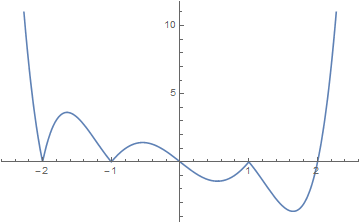
\includegraphics[scale=1]{eq}
\item[c) ] Hitta minsta värdet hos: $f(x) = x^4-4 x^2-2$

\end{itemize}

\subsection*{4}
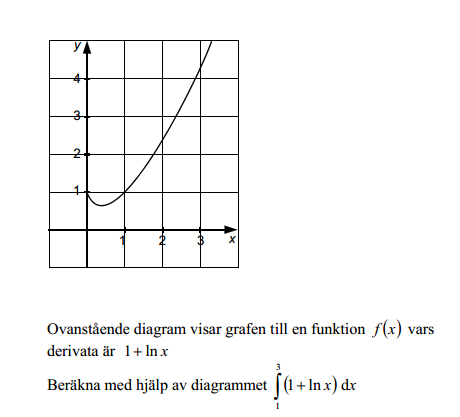
\includegraphics[scale=1]{primfunc}
\\
\textit{Nationellt prov Matematik D, VT-2002}

\subsection*{5}
\begin{itemize}
    \item[a) ] $\int_{-2}^2 (x+2) dx$
    \item[b) ] $\int_{- \pi}^{\pi} sin(x^3) dx$ 
    \item[c) ] $\int_1^2 (\frac{2}{x^3} - \frac{x^3}{2}) dx$
\end{itemize}

\subsection*{6}
\begin{itemize}
    \item[a) ] $\int \frac{cos x}{4 + sin^2 x} dx$ 
    \item[b) ] $\int x^2*2^{x^3+1} dx$ 
    \item[c) ] $\int \frac{dx}{x^2 + 6x +13}$ 
\end{itemize}

\end{document}
